\chapter{Supplemental Materials}
\label{supplementals}

To do.

% Software list/table
% DeepLabCut \href{https://github.com/DeepLabCut/DeepLabCut}
% MWorks \href{https://mworks.github.io}
% ScanImage 2016 \href{http://scanimage.vidriotechnologies.com}

\section{Supplementary Tables}

% Custom software
\href{https://github.com/coxlab/behavior_rig}
\href{https://github.com/julianarhee/morph-pov}

\href{https://github.com/julianrhee/retinotopy-mapper}
\href{https://github.com/julianarhee/acquisition-tools}

% Data numbers 

\begin{table}[h]
 \caption{Data Summary}
  \centering
   \begin{tabular}{lllll}
    \toprule
    Stimulus & Area & Rats & FOVs & Cells   \\
    \midrule
    Moving bar & V1  & 5 & 12 & 1277        \\
               & LM  & 6 & 14 & 530         \\
               & LI  & 4 & 9 & 502          \\
    \midrule
    Receptive Fields & V1  & 11 & 11 & 548  \\
                     & LM  & 8 & 8 & 241   \\
                     & LI  & 10 & 10 & 279    \\
    \midrule
    Gratings & V1  & 7 & 7 & 2211     \\
             & LM  & 8 & 8 & 2084     \\
             & LI  & 7 & 7 & 966     \\
    \midrule
    Objects  & V1  & 9 & 8 & 1028   \\
             & LM  & 10 & 7 & 684   \\
             & LI  & 8 & 7 & 402    \\
    \bottomrule
  \end{tabular}
  \label{tab:data_counts}
\end{table}


\section{Supplementary Figures}


% \section{Related to Chapter 1}
\begin{figure}[t!]
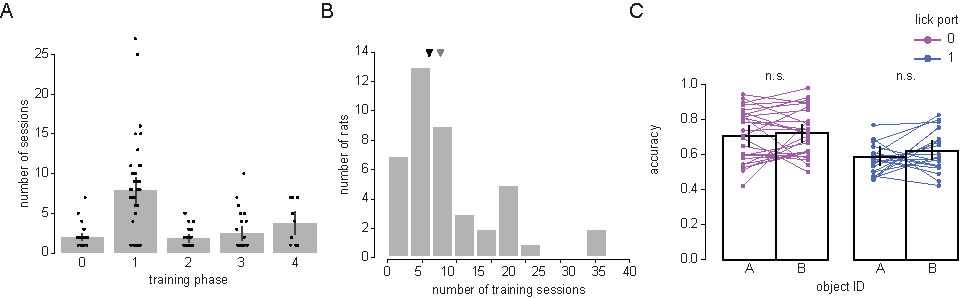
\includegraphics[width=\textwidth]{figures/supplemental/fig_s1_aggregate_training/fig_s1_aggregate_training.pdf}
    \vspace{.1in}
    \caption[Aggregate training data]{Aggregate training data. 
    \textbf{A.} Number of sessions per training phase. Each dot represents one rat. Bars show mean and SD.
    \textbf{B.} Histogram of the total number of training sessions to reach criterion (across all phases). Black and gray triangles denote the mean and median, respectively. 
    \textbf{C.} Accuracy split by object identity (object 1 or object 2) and port mapping (whether to lick right for object 1 and lick left for object 2, or vice versa). Each pair of lines represents one rat. Colors indicate arbitrary port assignment for the standard 2-object class paradigm. 
    \label{supfig:aggregate_training}}
\end{figure}


% FIGURE S.2 MORPH
\begin{figure}[t!]
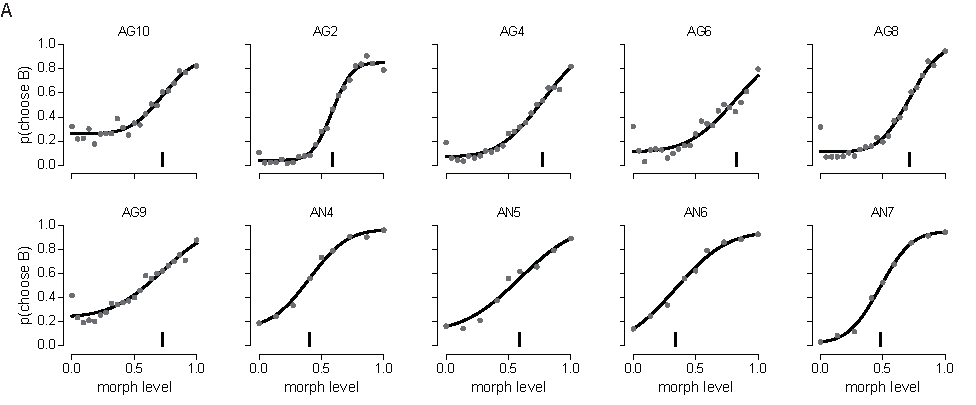
\includegraphics[width=\textwidth]{figures/supplemental/fig_s2_morphs_per_animal/fig_s2_morphs_per_animal.pdf}
    \vspace{.1in}
    \caption[Individual psychometric curves]{Individual psychometric curves for morphs. 
    \textbf{A.} Example psychometric curves for n=10 out 13 rats that passed criterion performance (70\% accuracy on the basic discrimination of the anchors). Each dot represents the fraction of times the animal chose the ``B''-assigned port, where morph level 0 is 0\%B and morph level 100 is 100\%B. Solid curves are the fits, vertical lines indicate bias. 
    \label{supfig:morphs}}
\end{figure}

% FIGURE S.3 INVAR
\begin{figure}[t!]
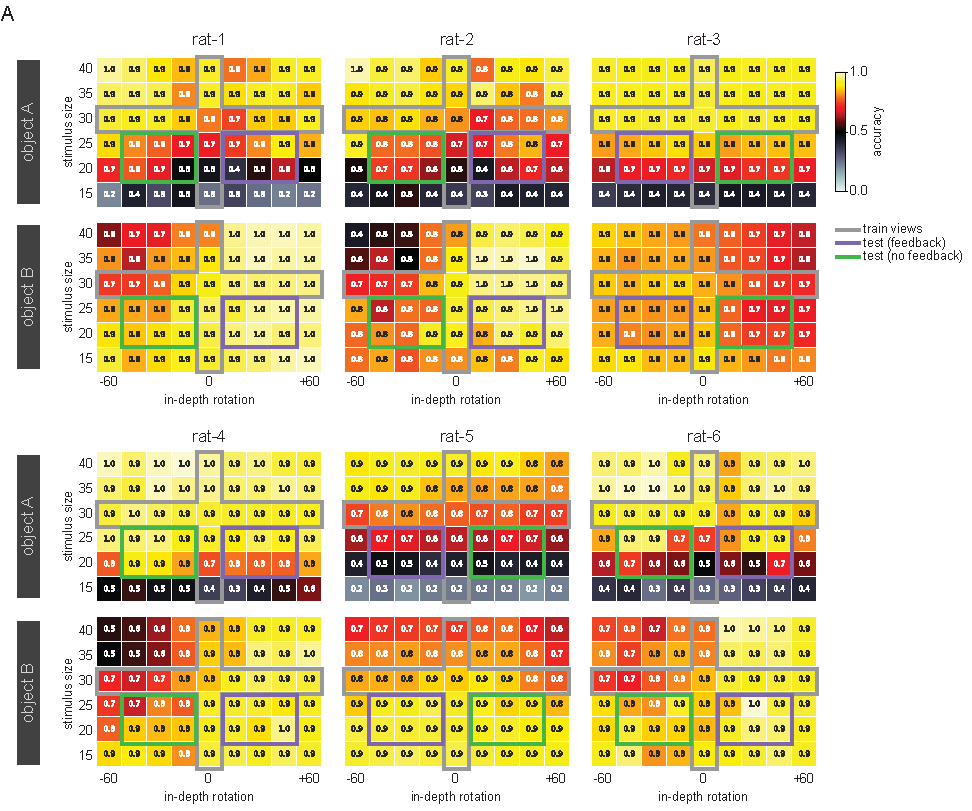
\includegraphics[width=\textwidth]{figures/supplemental/fig_s3_heatmaps_per_rat/fig_s3_heatmaps_per_rat.pdf}/
    \vspace{.1in}
    \caption[Individual invariance performance]{Individual performance on invariance test.
    \textbf{A.} Performance data for an example group of n=6 rats, split by object ID (top=object A, bottom=object B) and stimulus transformation. Colormap indicates accuracy. Gray, initial training views (views in which only a single transformation axis changes, size or rotation). Purple, views for which no feedback was provided. Green, size-matched view for which feedback was provided. 
    \label{supfig:heatmaps}}
\end{figure}

% \section{Related to Chapter 3}
% FIGURE S.4 STIMULI
\begin{figure}[t!]
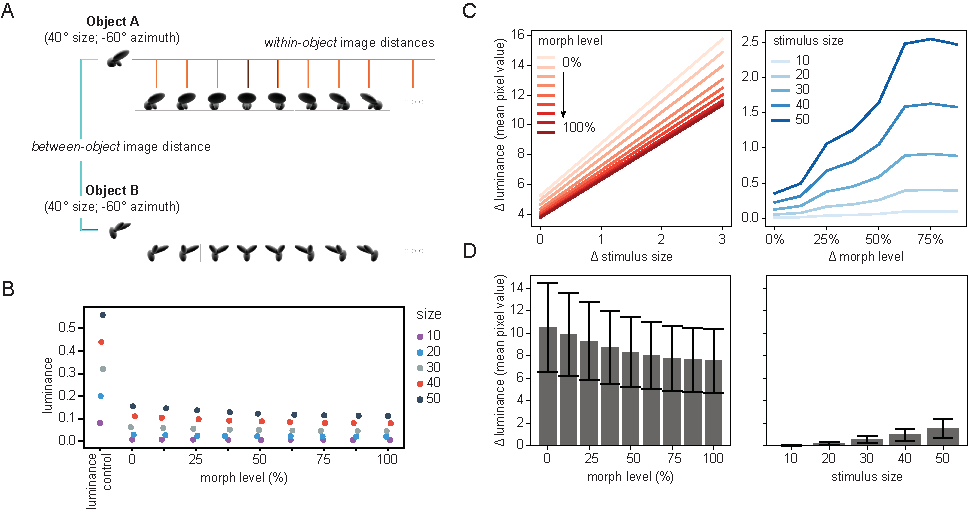
\includegraphics[width=\textwidth]{figures/supplemental/fig_s4_stimulus_metrics/fig_s4_stimulus_metrics.pdf}
    \vspace{.1in}
    \caption[Stimulus metrics]{Metrics defining the differences between images.
    \textbf{A.} The two objects were specified to have larger within-object distances than between-object distances at a given view (adapted from \cite{Zoccolan2009}). Distance was calculated as the Euclidean distance between the images. 
    \textbf{B.} Global mean luminance for each object image used for two-photon experiments, calculated as the average pixel value across the screen (image was transformed to screen coordinates), normalized by the max luminance value (255). Images are subsets of the images used to test behavior in trained rats. Luminance controls were full field stimuli (no shapes) assigned constant grayscale values that were experimentally determined to match photometer measurements of the screen at each stimulus size (placed at the position of the animal's eye). 
    \textbf{C.} \textit{Left}: Within-morph differences across different sizes. For each morph image, this was calculated as the pixel-wise difference between the morph at size \textit{s1} and the same morph at size \textit{s2}, for each pair of neighboring sizes. Level 1 represents the two smallest sizes, while level 4 represents the two largest sizes. Shades of red correspond to morph levels ordered from 0\%B to 100\%B. |textit{Right}:  Between-morph differences at each size. For each size (shades of blue), this was calculated as the pixel-wise difference between morph \textit{m0} at size \textit{s} and morph \textit{m1} at the same size, for each neighboring morph. Differences are greater at larger sizes.
    \textbf{D.}. Average within-morph differences (across size) for each morph tested (left), and average between-morph differences (across morph levels) for each size tested (right).    
    \label{supfig:stimulus_metrics}}
\end{figure}

% Visual field targeting
\begin{figure}[t!]
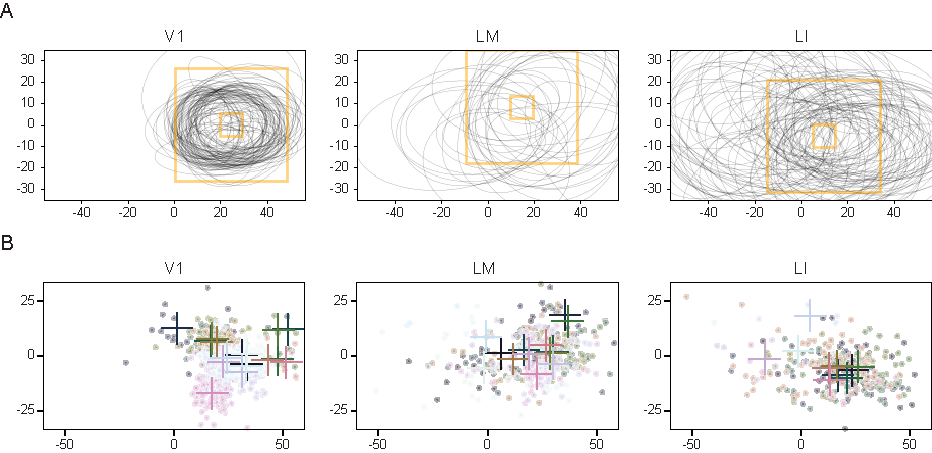
\includegraphics[width=\textwidth]{figures/supplemental/fig_s5_vf_targeting/fig_s5_vf_targeting.pdf}
    \vspace{.1in}
    \caption[Visual Field Targeting]{Target visual stimulation with receptive field mapping.
    \textbf{A.} The two objects were specified to have larger within-object distances than between-object distances at a given view (adapted from \cite{Zoccolan2009}). Distance was calculated as the Euclidean distance between the images. 
    \label{supfig:vf_targeting}}
\end{figure}


% \subsection{Comparison of stimulus size for receptive field measurements}
\begin{figure}[t!]
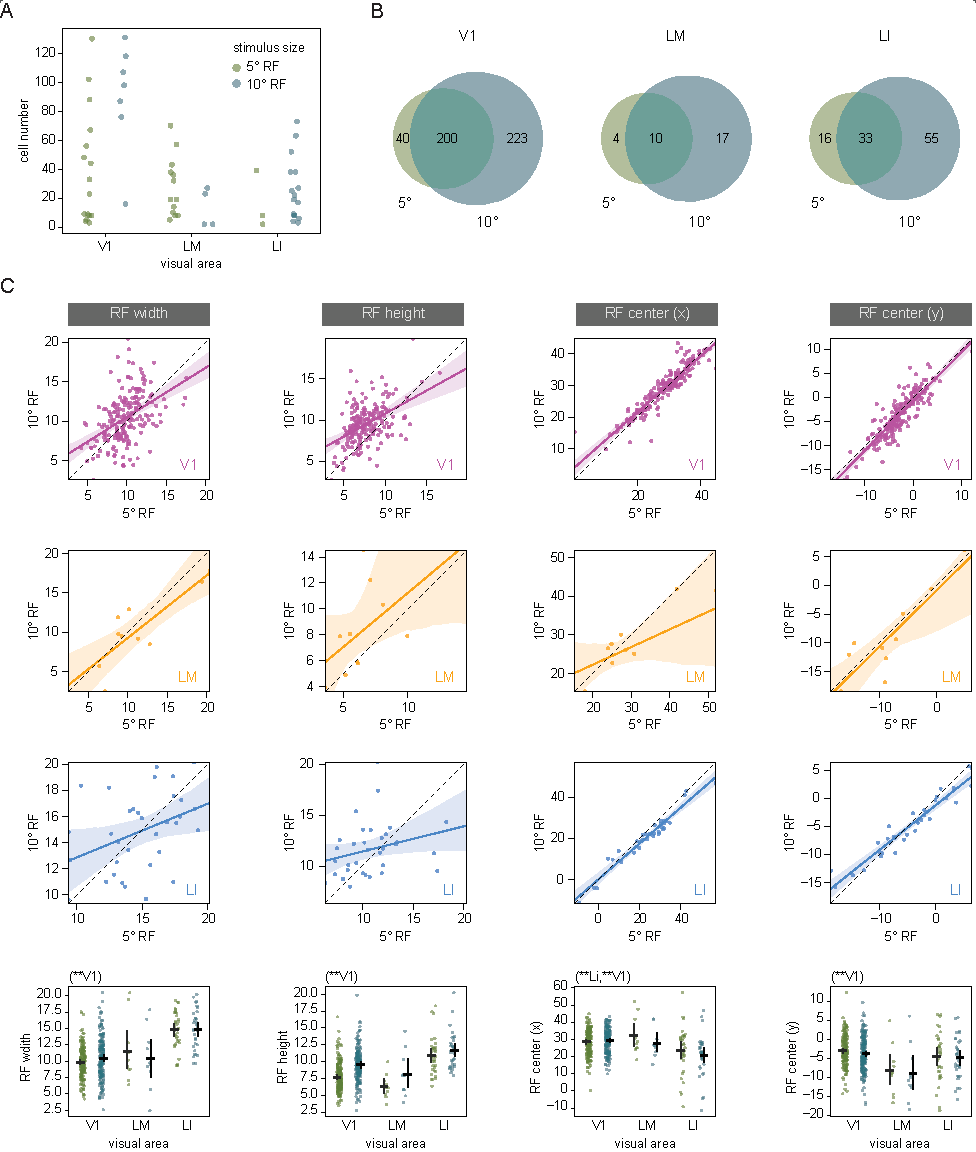
\includegraphics[width=\textwidth]{figures/supplemental/fig_s6_rf5_v_rf10/fig_sX_rf5_rf10.pdf}
    \vspace{.1in}
    \caption[RF mapping stimuli]{Effect of stimulus size for RF measurements.
    \textbf{A.} The two objects were specified to have larger within-object distances than between-object distances at a given view (adapted from \cite{Zoccolan2009}). Distance was calculated as the Euclidean distance between the images. 
    \label{supfig:rf5_rf10}}
\end{figure}


% \subsection{Demonstration of spherical correction}
\begin{figure}[t!]
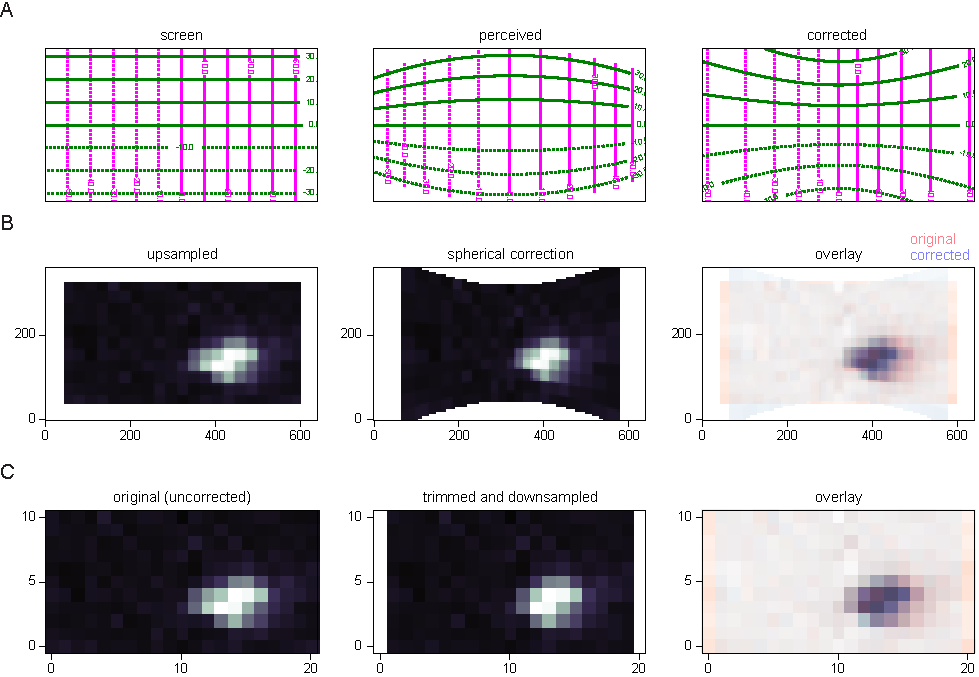
\includegraphics[width=\textwidth]{figures/supplemental/fig_sX_spherical_correction_steps/fig_sX_spherical_correction_steps.pdf}
    \vspace{.1in}
    \caption[Spherical correction]{Steps for posthoc spherical correction.
    \textbf{A.} The two objects were specified to have larger within-object distances than between-object distances at a given view (adapted from \cite{Zoccolan2009}). Distance was calculated as the Euclidean distance between the images. 
    \label{supfig:spherical_correction_steps}}
\end{figure}

% \subsection{Demonstration of spherical correction}
\begin{figure}[t!]
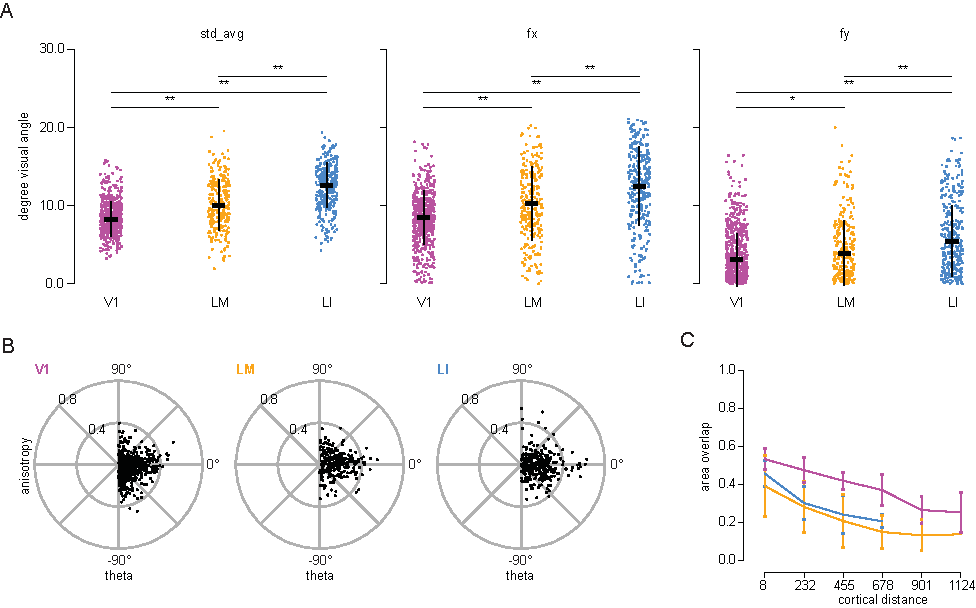
\includegraphics[width=\textwidth]{figures/supplemental/fig_sX_spherical_correction_aggregate/fig_sX_spherical_correction_aggregate.pdf}
    \vspace{.1in}
    \caption[Spherical correction]{Steps for posthoc spherical correction.
    \textbf{A.} The two objects were specified to have larger within-object distances than between-object distances at a given view (adapted from \cite{Zoccolan2009}). Distance was calculated as the Euclidean distance between the images. 
    \label{supfig:spherical_correction_aggregate}}
\end{figure}

% \begin{figure}[t!]
% \includegraphics[width=\textwidth]{figures/supplemental/fig_sX_spherical_correction_examples/fig_sX_spherical_correction_examples.pdf}
%     \vspace{.1in}
%     \caption[Spherical correction]{Steps for posthoc spherical correction.
%     \textbf{A.} The two objects were specified to have larger within-object distances than between-object distances at a given view (adapted from \cite{Zoccolan2009}). Distance was calculated as the Euclidean distance between the images. 
%     \label{supfig:spherical_correction_examples}}
% \end{figure}

% \subsection{Comparison of receptive field and gratings tuning}
\begin{figure}[t!]
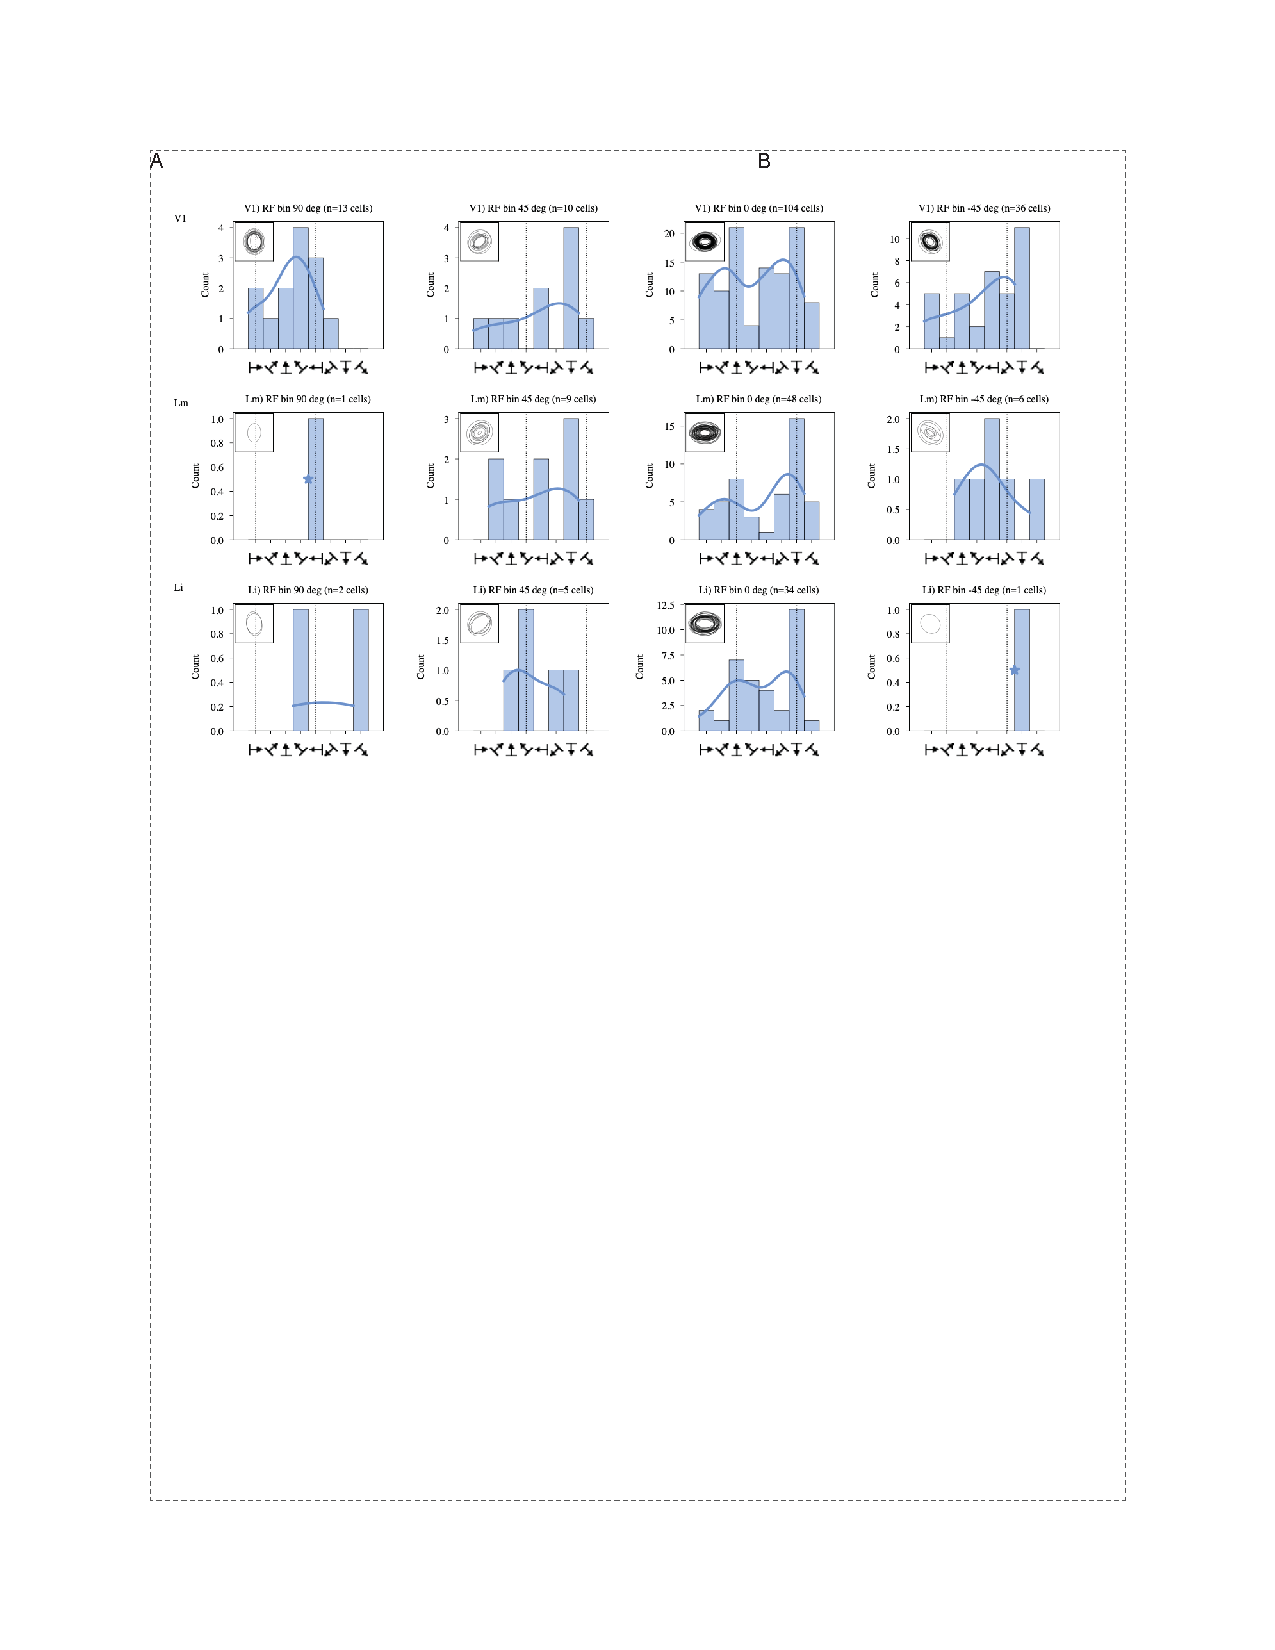
\includegraphics[width=\textwidth]{figures/supplemental/fig_sX_theta_vs_rf/fig_sX_theta_vs_rf.pdf}
    \vspace{.1in}
    \caption[Receptive field shape and Direction tuning]{Axis selectivity by receptive field orientation.
    \textbf{A.} The two objects were specified to have larger within-object distances than between-object distances at a given view (adapted from \cite{Zoccolan2009}). Distance was calculated as the Euclidean distance between the images. 
    \label{supfig:theta_vs_rf}}
\end{figure}



% \section{Related to Chapter 4}

% \subsection{Tuning similarity as a function of distance}

% \subsection{Classifier accuracy as a function of receptive overlap}

% \subsection{Classifier generalization, matched for receptive field size}
